%Asservissement par traitement d’image d’une plateforme Hexapode

\section*{Contexte}

La caractérisation du système squelettique humain est une donnée importante pour la mise en place de traitements
dédiés en cas de troubles musculo-squelettiques. Des études sur ce sujet existent en utilisant des modélisations
mécaniques de la colonne vertébrale et des simulations numériques par la méthode des éléments finis
par exemple.

Cependant, la validation de ces modèles nécessite la mise en place d’essais expérimentaux. Un dispositif expérimental
étudié par certaines équipes de recherche est organisé autour d’un Hexapode piloté en position. Ce
dispositif est représenté sur la \autoref{fig:01} Le pilotage de la plateforme supérieure est souvent réalisé en asservissant
directement les positions des différents axes. Ce choix technique permet une réalisation facile de la chaine de
commande mais possède un inconvénient : il entraine un manque de précision en raison de la souplesse des vérins
et des jeux dans les liaisons de l’Hexapode.

\begin{figure}[H]
\centering
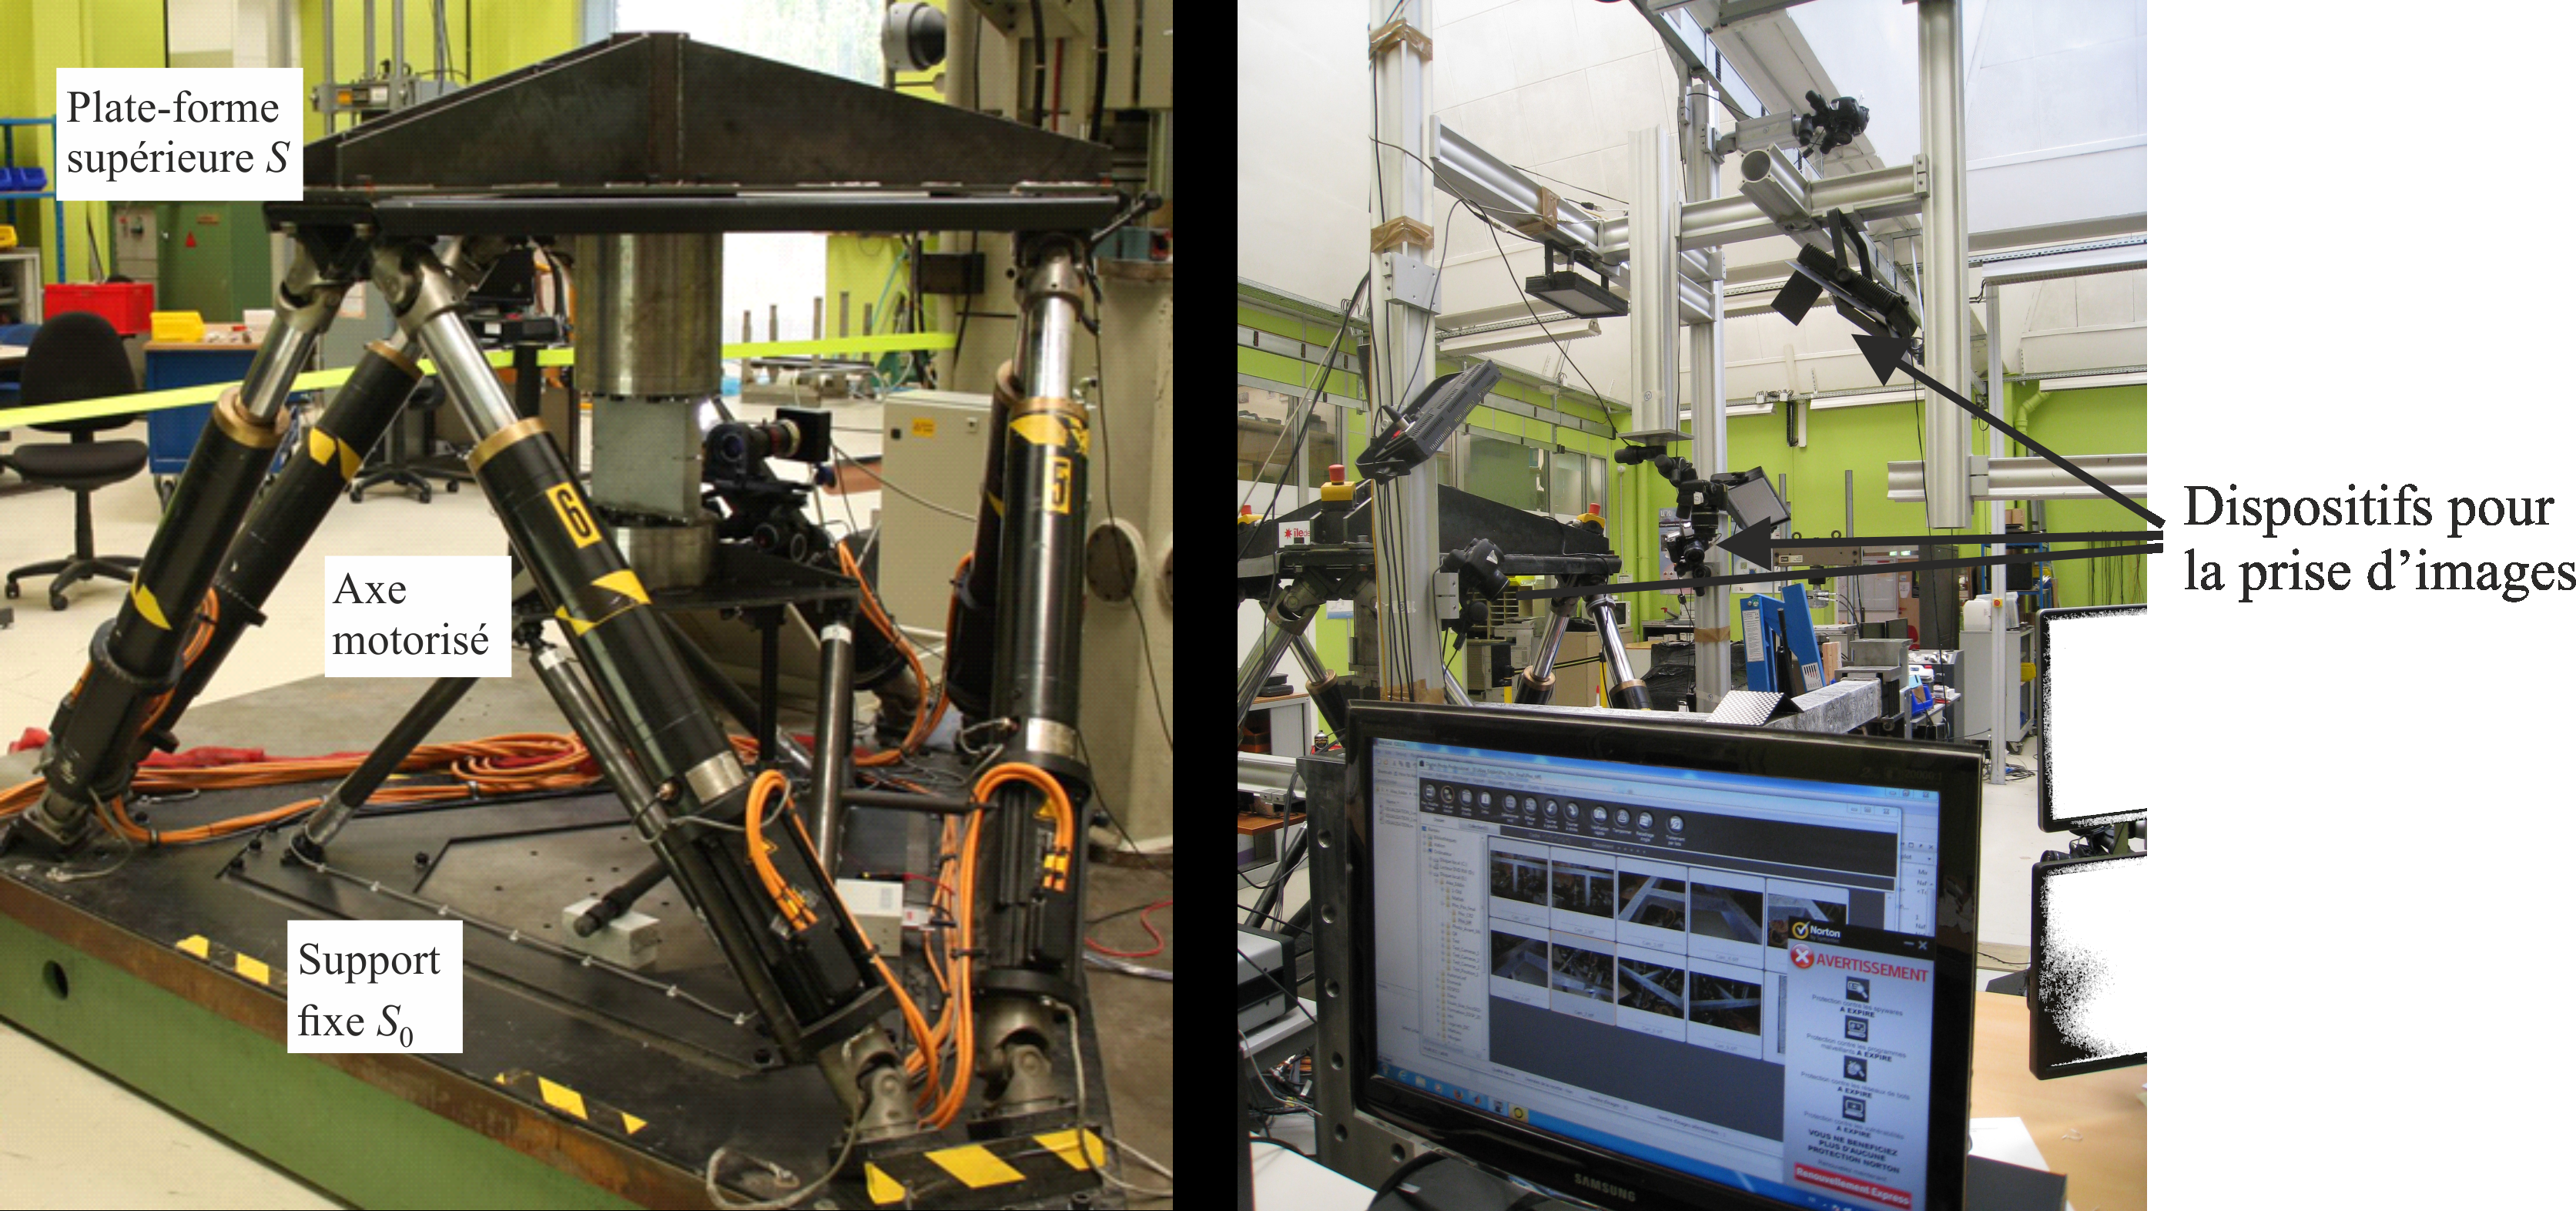
\includegraphics[width=.8\linewidth]{fig_01}
\caption{\label{fig:01} Système d’asservissement en position d’un Hexapode par traitement d’images}
\end{figure}



L’architecture de commande de l’Hexapode est représentée par le schéma de la figure 2. Une des solutions
consiste à asservir les longueurs des vérins $L_i$ à des longueurs de référence $L_i^*$ 
obtenues en utilisant un modèle cinématique inverse à partir des positions souhaitées $P_i^*$ 
de la plateforme dans un repère absolu. Une solution
simple pour déterminer les longueurs des vérins est d’utiliser des mesures issues de capteurs montés directement
sur les axes des moteurs (en tenant compte du rapport de transmission). Mais la simplicité de cette solution
peut conduire à des erreurs en raison de la souplesse des tiges du vérin, ou encore des jeux dans les liaisons,
conduisant ainsi à une longueur de vérin $L_i^d$ 
différente de celle mesurée $L_i^m$. Dans ce contexte, la \autoref{fig:02} propose
deux solutions possibles :
\begin{itemize}
\item la première solution utilise une loi de commande exploitant les seules mesures $L_i^m$ issues des capteurs montés
sur les vérins et entachées d’erreurs dues à la souplesse des tiges et aux jeux éventuels ;
\item une deuxième solution, plus évoluée, exploite une estimation des positions réelles $L_i^{de}$ des extrémités des tiges
des vérins. Une méthode permettant d’obtenir cette estimation est d’utiliser une caméra et un algorithme
de traitement d’images.
\end{itemize}
L’objet de ce sujet est d’évaluer ces solutions et de déterminer une loi de commande permettant d’obtenir
un positionnement de la plateforme selon le cahier des charges représenté sur la figure 3 sous la forme d’un
diagramme des exigences. Ce sujet est décomposé en trois parties :
\begin{itemize}
\item dans la \autoref{sec:01}, il s’agira de développer un modèle mécanique (cinématique) de l’axe ;
\item dans la \autoref{sec:02}, une étude de la précision des axes motorisés sera réalisée en utilisant le modèle développé
dans la \autoref{sec:01} ;
\item enfin dans la \autoref{sec:03}, il s’agira de définir les éléments de l’algorithme de traitement d’images permettant
d’estimer les longueurs réelles des tiges du vérin et de développer des lois de commande permettant d’asservir
la position de la plateforme à une position de référence associée à l’essai à réaliser.
\end{itemize}


\begin{figure}[H]
\centering
\includegraphics[width=.8\linewidth]{fig_02}
\caption{\label{fig:02} Architecture de commande de l’Hexapode }
\end{figure}


\begin{figure}[H]
\centering
\includegraphics[width=.8\linewidth]{fig_03}
\caption{\label{fig:03} Diagramme des exigences }
\end{figure}



\section{\label{sec:01} Étude cinématique de la plateforme Hexapode}

\begin{obj}
Le but de cette partie est d’étudier les mouvements de la plateforme Hexapode afin de définir le modèle
cinématique inverse permettant de déterminer la longueur à imposer aux axes motorisés pour vérifier
un positionnement donné de la plateforme mobile.
\end{obj}
La plateforme Hexapode utilisée ici est constituée des composants suivants, représentés sur les \autoref{fig:04} et \autoref{fig:05} :
\begin{itemize}
\item un support $S_0$, de forme triangulaire, parfaitement lié au sol, et que l’on assimilera au bâti ;
\item une plateforme mobile $S$, de forme triangulaire, dont la mise en position permettra de solliciter expérimentalement
la colonne vertébrale dont l’une des extrémités lui est fixée rigidement ;
\item six axes rectilignes motorisés dont la longueur peut être pilotée, et reliés au niveau de leurs extrémités par
des liaisons sphériques au support $S_0$ d’un côté, à la plateforme $S$ de l’autre.
\end{itemize}

\subsection{ Mouvement d’un axe motorisé (seul) par rapport au support}



\begin{obj}
L’objectif de cette sous-partie est de déterminer les degrés de liberté d’un axe motorisé (seul) par
rapport au support.
\end{obj}

Chaque axe motorisé présente l’architecture illustrée sur la \autoref{fig:04} :
\begin{itemize}
\item un ensemble \{support moteur (13) + corps de vérin (10)\}, relié au support fixe par l’intermédiaire d’une
liaison que l’on peut modéliser par une liaison sphérique (rotule inférieure (14)) ;
\item un ensemble \{actionneur électrique (1) + réducteur (2)\}, fixé au corps de vérin (10) et entrainant la vis (4)
en rotation autour de son axe ;
\item un écrou (5) en liaison par rapport au corps de vérin (10) modélisable par une liaison glissière et en liaison
hélicoïdale par rapport à la vis (4) ;
\item une tige de vérin (7), solidaire de l’écrou (5), et reliée à son extrémité avec la plateforme mobile par l’intermédiaire
d’une liaison que l’on peut modéliser comme une liaison sphérique (rotule supérieure (8)).
\end{itemize}



\begin{figure}[H]
\centering
\includegraphics[width=.8\linewidth]{fig_04}
\caption{\label{fig:04}  }
\end{figure}


%Q01
\question{\label{q:01}À l’aide des informations précédentes, compléter sur le document réponse (figure A) le schéma cinématique
(plan) d’un axe motorisé, en repérant, à l’aide de plusieurs couleurs, l’ensemble \{corps de vérin (10) +
support moteur (13)\}, l’ensemble \{tige de vérin (7) + ecrou (5)\} et la vis (4). On ne tiendra pas compte du
système \{roue (12) + vis sans fin (3)\} associé au capteur (11).}
\ifprof
\begin{corrige}
\end{corrige}
\else
\fi


%Q02
\question{\label{q:02}Déterminer par une méthode à choisir la liaison cinématiquement équivalente à l’ensemble des trois
liaisons présentes entre la tige de vérin (7) et le corps de vérin (10). Représenter sur le document réponse le
schéma cinématique du nouveau modèle (avec la liaison équivalente).}
\ifprof
\begin{corrige}

\end{corrige}
\else
\fi


%Q03
\question{\label{q:03}Déterminer l’expression littérale du vecteur vitesse $\vectv{A}{7}{S_0}$ dans la base $\base{x_1}{y_1}{z_1}$. Combien de
paramètres de mouvement sont alors nécessaires et suffisants pour positionner le point $A$ (centre de la rotule
supérieure (8)) par rapport à $S_0$ ?}
\ifprof
\begin{corrige}

\end{corrige}
\else
\fi



\subsection{Mouvement de la plateforme $S$ par rapport au support $S_0$}

\begin{obj}
L’objectif de cette sous-partie est d’étudier le mouvement de la plateforme en vue de la réalisation
d’un essai spécifique.
\end{obj}


L’architecture de la plateforme Hexapode est représentée sur la \autoref{fig:05} :
\begin{itemize}	
\item au support fixe $S_0$ est attaché le référentiel $\rep{0}\repere{O}{x_0}{y_0}{z_0}$ supposé galiléen, où $\left(O,\vect{x_0},\vect{y_0}\right)$ est le plan
contenant les points $D$, $E$ et $F$;
\item à la plateforme mobile $S$ est attaché le référentiel $\rep{}\repere{G}{x}{y}{z}$ , où $\left(G,\vect{x},\vect{y}\right)$ est le plan contenant les points
$A$,$B$ et $C$;
\item chaque axe $i$ ($1\leq i \leq 6$), relie un point de la plateforme $S$ à un point du support $S_0$ : $\vect{DA}=L_1\vect{u_1}$,
$\vect{DB}=L_2\vect{u_2}$, 
$\vect{EB}=L_3\vect{u_3}$,
$\vect{EC}=L_4\vect{u_4}$,
$\vect{FC}=L_5\vect{u_5}$ et
$\vect{FA}=L_6\vect{u_6}$ où les vecteurs $\vect{u_i}$ sont unitaires.
\end{itemize}

\begin{figure}[H]
\centering
\includegraphics[width=.4\linewidth]{fig_05}
\caption{\label{fig:05} Architecture de la plateforme Hexapode (les liaisons équivalentes
entre tiges et corps de vérins ne sont pas représentées). }
\end{figure}

%Q04
\question{\label{q:04} À l’aide du nombre de paramètres de mouvement (déterminé à la question \ref{q:03}) du centre de la rotule
supérieure de chaque axe motorisé et du nombre de relations scalaires indépendantes que l’on peut écrire à
propos des positions de ces centres, montrer que la plateforme mobile $S$ a six degrés de liberté par rapport au
support $S_0$.}
\ifprof
\begin{corrige}
\end{corrige}
\else
\fi

Dans la suite, on choisira comme degrés de liberté les trois coordonnées cartésiennes de la position du centre de
gravité $G\left(x_G,y_G,z_G\right)_{\rep{0}}$ de la plateforme mobile $S$ dans $\rep{0}$, ainsi que les trois angles d’Euler $\left(\psi, \theta, \phi\right)$ définis
dans la \autoref{fig:06}.

Afin de pouvoir solliciter la colonne vertébrale testée, la plateforme mobile $S$ doit pouvoir être pilotée de façon à
ce que le triangle ABC soit contenu dans un plan ($\Pi$) dont l’équation cartésienne dans $\rep{0}$ est ($\Pi$) : $z=ax+by+c$
où $\left(x,y,z\right)$ sont les coordonnées dans $\rep{0}$ d’un point $M$ de ($\Pi$) et $(a,b,c)$ sont trois constantes non nulles.

\begin{figure}[H]
\centering
\includegraphics[width=.8\linewidth]{fig_06}
\caption{\label{fig:06} Définition des trois angles d’Euler (précession $\psi$, nutation $\theta$, rotation propre $\phi$).}
\end{figure}


%Q05
\question{\label{q:05} Déterminer l’équation cartésienne dans $\rep{0}$ du plan de la plateforme mobile $S$ à l’aide des six degrés
de liberté $\left( x_G,y_G,z_G, \psi, \theta, \phi \right)$de cette dernière. Pour cela, on calculera le produit scalaire 
$\vect{GM}\cdot \vect{n}$, où $\vect{n}$ est le
vecteur normal unitaire à la plateforme mobile que l’on exprimera à l’aide des vecteurs de la base $\base{x}{y}{z}$. En
déduire qu’il est possible de relier les degrés de liberté $\left( x_G,y_G,z_G, \psi, \theta\right)$ de la plateforme mobile $S$ aux constantes
$\left(a,b,c\right)$ de l’équation cartésienne de ($\Pi$) ; on ne cherchera pas à expliciter les fonctions donnant l’expression de
$\left( x_G,y_G,z_G, \psi, \theta\right)$ en fonction de $\left(a,b,c\right)$. Pourquoi l’angle de rotation propre $\phi$ n’intervient-il pas dans l’équation
demandée ?}
\ifprof
\begin{corrige}
\end{corrige}
\else
\fi


%Q
\question{\label{q:}}
\ifprof
\begin{corrige}
\end{corrige}
\else
\fi


%Q
\question{\label{q:}}
\ifprof
\begin{corrige}
\end{corrige}
\else
\fi

%Q
\question{\label{q:}}
\ifprof
\begin{corrige}
\end{corrige}
\else
\fi


%Q
\question{\label{q:}}
\ifprof
\begin{corrige}
\end{corrige}
\else
\fi


%Q
\question{\label{q:}}
\ifprof
\begin{corrige}
\end{corrige}
\else
\fi


%Q
\question{\label{q:}}
\ifprof
\begin{corrige}
\end{corrige}
\else
\fi


%Q
\question{\label{q:}}
\ifprof
\begin{corrige}
\end{corrige}
\else
\fi


%Q
\question{\label{q:}}
\ifprof
\begin{corrige}
\end{corrige}
\else
\fi


%Q
\question{\label{q:}}
\ifprof
\begin{corrige}
\end{corrige}
\else
\fi


%Q
\question{\label{q:}}
\ifprof
\begin{corrige}
\end{corrige}
\else
\fi


%Q
\question{\label{q:}}
\ifprof
\begin{corrige}
\end{corrige}
\else
\fi


%Q
\question{\label{q:}}
\ifprof
\begin{corrige}
\end{corrige}
\else
\fi


%Q
\question{\label{q:}}
\ifprof
\begin{corrige}
\end{corrige}
\else
\fi


%Q
\question{\label{q:}}
\ifprof
\begin{corrige}
\end{corrige}
\else
\fi


%Q
\question{\label{q:}}
\ifprof
\begin{corrige}
\end{corrige}
\else
\fi


%Q
\question{\label{q:}}
\ifprof
\begin{corrige}
\end{corrige}
\else
\fi


%Q
\question{\label{q:}}
\ifprof
\begin{corrige}
\end{corrige}
\else
\fi


%Q
\question{\label{q:}}
\ifprof
\begin{corrige}
\end{corrige}
\else
\fi


%Q
\question{\label{q:}}
\ifprof
\begin{corrige}
\end{corrige}
\else
\fi


%Q
\question{\label{q:}}
\ifprof
\begin{corrige}
\end{corrige}
\else
\fi


%Q
\question{\label{q:}}
\ifprof
\begin{corrige}
\end{corrige}
\else
\fi


%Q
\question{\label{q:}}
\ifprof
\begin{corrige}
\end{corrige}
\else
\fi


%Q
\question{\label{q:}}
\ifprof
\begin{corrige}
\end{corrige}
\else
\fi








\begin{figure}[H]
\centering
\includegraphics[width=.8\linewidth]{fig_07}
\caption{\label{fig:07}  }
\end{figure}


\begin{figure}[H]
\centering
\includegraphics[width=.8\linewidth]{fig_08}
\caption{\label{fig:08}  }
\end{figure}


\begin{figure}[H]
\centering
\includegraphics[width=.8\linewidth]{fig_09}
\caption{\label{fig:09}  }
\end{figure}


\begin{figure}[H]
\centering
\includegraphics[width=.8\linewidth]{fig_10}
\caption{\label{fig:10}  }
\end{figure}


\begin{figure}[H]
\centering
\includegraphics[width=.8\linewidth]{fig_11}
\caption{\label{fig:11}  }
\end{figure}

\begin{figure}[H]
\centering
\includegraphics[width=.8\linewidth]{fig_12}
\caption{\label{fig:12}  }
\end{figure}

\begin{figure}[H]
\centering
\includegraphics[width=.8\linewidth]{fig_13}
\caption{\label{fig:13}  }
\end{figure}

\begin{figure}[H]
\centering
\includegraphics[width=.8\linewidth]{fig_14}
\caption{\label{fig:14}  }
\end{figure}
